\documentclass[a4paper,UKenglish]{lipics-v2016}


\usepackage{microtype}



\bibliographystyle{plain}

\usepackage{pgf, tikz}
\usetikzlibrary{arrows, automata, petri}

\usepackage{longtable}

\usepackage{algorithm}
\usepackage[noend]{algpseudocode}


\title{The \io complexity of Strassen's matrix multiplication
  with recomputation}
\titlerunning{The \io complexity of Strassen's matrix multiplication
  with recomputation} 

\author[1]{Gianfranco Bilardi}
\author[2]{Lorenzo De Stefani}
\affil[1]{Department of Information Engineering, University of Padova, Via Gradenigo 6B/Padova, Italy\\
  \texttt{bilardi@dei.unipd.it}}
\affil[2]{Department of Computer Science, Brown University, 115 Waterman Street/Providence, United States of America\\
  \texttt{lorenzo@cs.brown.edu}}
\authorrunning{G. Bilardi and L. De Stefani} 

\Copyright{Gianfranco Bilardi and Lorenzo De Stefani}

\subjclass{F.2.1 Numerical Algorithms and Problems}\keywords{\io complexity,  Strassen's Matrix Multiplication, Recomputation, Memory Hierarchy, Parallel Computation}

\newcommand{\ri}{\mathcal{R}}
\newcommand{\BO}[1]{\mathcal{O}\left(#1\right)}
\newcommand{\BOme}[1]{\Omega\left(#1\right)}

\newcommand{\io }{I/O }
\newcommand{\stral}[1]{\mathcal{H}^{#1}}
\newcommand{\alg}{\mathcal{A}}




\begin{document}

\maketitle

\begin{abstract}
A tight  lower bound is derived on
the \io complexity of Strassen's algorithm to multiply two  matrices, in a two-level storage hierarchy with  words of fast
memory.  A proof technique is introduced, which exploits the Grigoriev's
flow of the matrix multiplication function as well as some
combinatorial properties of the Strassen computational directed acyclic graph (CDAG).
Applications to parallel computation are also developed. The result
generalizes a similar bound previously obtained under the constraint
of no-recomputation, that is, that intermediate results cannot be
computed more than once. For this restricted case, another lower bound
technique is presented, which leads to a simpler analysis of the \io
complexity of Strassen's algorithm and can be readily extended to
other ``Strassen-like'' algorithms.
 \end{abstract}

\section{Introduction}
Data movement is increasingly playing a major role in the performance
of computing systems, in terms of both time and energy. This current
technological trend~\cite{patterson2005getting} is destined to
continue, since the very fundamental physical limitations on minimum
device size and maximum message speed lead to inherent costs when
moving data, whether across the levels of a hierarchical memory system
or between processing elements of a parallel
systems~\cite{bilardi1995horizons}. The communication requirements of
algorithms have been the target of considerable research in the last
four decades; however, obtaining significant lower bounds based on such
requirements remains and important and challenging task.

In this paper we focus on the \io complexity of Strassen's matrix
multiplication algorithm.  Matrix multiplication is a pervasive
primitive utilized in many applications.
Strassen~\cite{strassen1969gaussian} showed that two 
matrices can be multiplied with , with , hence with asymptotically fewer than the 
arithmetic operations required by the straightforward implementation
of the definition of matrix multiplication. This result has motivated
a number of efforts which have lead to increasingly faster algorithms,
at least asymptotically, with the current record being at ~\cite{legall2014}.

\paragraph*{Previous and related work}

\io complexity has been introduced in the seminal work by Hong and
Kung~\cite{jia1981complexity}; it is essentially the number of data
transfers between the two levels of a memory hierarchy with a fast
memory of  words and a slow memory with an unbounded number of
words. They presented techniques to develop lower bounds to the \io
complexity of computations modeled by \emph{computational directed acyclic graphs} (CDAGs). The resulting lower bounds
apply to all the schedules of the given CDAG, including those with
recomputation, that is, where some vertices of the CDAG are evaluated
multiple times. Among other results, they established an  lower bound to the \io complexity of the definition-based
matrix multiplication algorithm, which matched a known upper bound
upper bound~\cite{cannon1969cellular}. The techniques
of~\cite{jia1981complexity} have also been extended to obtain tight
communication bounds for the definition-based matrix multiplication in
some parallel settings~\cite{irony2004communication,frigo1999cache}.

Ballard et al.  generalized the results on matrix multiplication of
Hong and Kung~\cite{jia1981complexity} in~\cite{ballard2011minimizing,
  ballard2010communication} by using the approach proposed
in~\cite{irony2004communication} based on the Loomis-Whitney geometric
theorem~\cite{loomis1949,zalg}. The same papers presents tight \io
complexity bounds for various classical linear algebra algorithms, for
problems such as LU/Cholesky/LDLT/QR factorization and eigenvalues and
singular values computation. 


It is natural to wonder what is the impact of Strassen's reduction of
the number of arithmetic operations on the number of data transfers.
In an important contribution Ballard et
al.~\cite{ballard2012graph}, obtained an
 \io lower bound for Strassen's
algorithm, using the ``\emph{edge expansion approach}''. The authors
extend their technique to a class of ``\emph{Strassen-like}'' fast
multiplication algorithms and to fast recursive multiplication
algorithms for rectangular matrices~\cite{ballard2012graphrec}. This
result was later generalized to a broader class of
``\emph{Strassen-like}'' algorithms of by Scott
et. al~\cite{scott2015matrix} using the ``\emph{path routing}''
technique.  A parallel, ``\emph{communication avoiding}''
implementation of Strassen's algorithm whose performance matches the
known lower bound~\cite{ballard2012graph,scott2015matrix}, was
proposed by Ballard et al.~\cite{ballard2012communicationalg}.

The edge expansion technique of~\cite{ballard2012graph}, the path
routing technique of~\cite{scott2015matrix}, and the ``\emph{closed dichotomy
width}'' technique of~\cite{bilardi1999processor} all yield \io lower
bounds that apply only to computational schedules for which no
intermediate result is ever computed more than once
(\emph{nr-computations}). 
While it is of interest to know what is the
\io complexity achievable by nr-computations, it is also
important to investigate what can be achieved with recomputation. In
fact, for some CDAGs, recomputing intermediate values does reduce the
space and/or the \io complexity of an
algorithm~\cite{savage1995extending}.
In~\cite{bilardi2001characterization}, it is shown that some
algorithms admit a \emph{portable schedule} (i.e., a schedule which
achieves optimal performance across memory hierarchies with different
access costs) only if recomputation is allowed. A number of lower
bound techniques that allow for recomputation have been presented in
the literature, including the ``\emph{S-partition}
technique''~\cite{jia1981complexity}, the ``\emph{S-span}
technique''~\cite{savage1995extending}, and the ``\emph{S-covering}
technique''~\cite{bilardi2000space} which merges and extends aspects
from both~\cite{jia1981complexity}
and~\cite{savage1995extending}. None of these has however been
successfully applied to fast matrix multiplication algorithms.

\paragraph*{Our results}

Our main result is the extension of the  \io complexity lower bound for Strassen's algorithm to
schedules with recomputation. A matching upper bound is known, and
obtained without recomputation; hence, we can conclude that, for
Strassen's algorithm, recomputation does not help in reducing \io
complexity if not, possibly, by a constant factor. In addition to the
result itself, the proof technique appears to be of independent
interest, since it exploits to a significant extent the
divide\&conquer nature which is exhibited by many algorithms.  We do
follow the dominator-set approach pioneered by Hong and Kung
in~\cite{jia1981complexity}. However, we focus the dominator analysis
only on a select set of target vertices, specifically the outputs of
the sub-CDAGs of Strassen's CDAG that correspond to sub-problems of a
suitable size (a size chosen as a function of the fast memory
capacity, ).  Any dominator set of a set of target vertices can be
partitioned into two subsets, one internal and one external to the
sub-CDAGs. The analysis of the external component of the dominator does
require rather elaborate arguments that are specific to Strassen's
CDAG. In contrast, the analysis of the internal component can be
carried out based only on the fact that the sub-CDAGs compute matrix
products, irrespective of the algorithm (in our case, Strassen's) by
which the products are computed.  To achieve this independence of the
algorithm, we resort on the concept of Grigoriev's flow of a
function~\cite{grigor1976application} and on a lower bound to such
flow established by Savage~\cite{savage97models} for matrix
multiplication.

As it turns out, for schedules without recomputation, the analysis of
the external component of the dominator sets becomes unnecessary and
the analysis of the internal components can be somewhat simplified.
The result is a derivation of the \io complexity without recomputation
considerably simpler than those in~\cite{ballard2012graph,
  scott2015matrix}.  The technique is easily extended to a class of
Strassen-like algorithms.

The paper is organized as follows: in Section~\ref{sec:preliminaries},
we provide the details of our model and of several theoretical notions
needed in our analysis. Section~\ref{sect:stranore} describes the
simplified lower bound for Strassen's and Strassen-like algorithms,
when implemented with no recomputation. In Section~\ref{sec:stragen}, we present
the \io complexity lower bound for Strassen's algorithm, when
recomputation is allowed. Extensions of the result to a parallel
model are also discussed.


\section{Preliminaries}\label{sec:preliminaries}
We consider algorithms which compute the product  of  matrices  with entries form a ring . Specifically, we
focus on algorithms whose execution, for any given , can be modeled
as a \emph{computational directed acyclic graph} (CDAG) ,
where each vertex  represents either an input value or the
result of an unit time operation (i.e.  an intermediate result or one
of the output values), while the directed edges in  represent data
dependences. A \emph{directed path} connecting vertices  is
an ordered sequence of vertices for which  and  are respectively
the first, and last vertex such that there is in  a (directed) edge
pointing from each vertex in the sequence to its successor. We say
that a CDAG  is a \emph{sub-CDAG} of  if
 and .
\paragraph*{Model}

We assume that sequential computations are executed on a system with a
two-level memory hierarchy consisting of a fast memory or \emph{cache}
of size , measured in words, and a \emph{slow memory} of
unlimited size. We assume that each memory word can store at most one
value form . An operation can be executed only if all its
operands are presents in cache. Data can be moved from the slow memory
to the cache by \emph{read} operations and in the other direction
by \emph{write} operations. Read and write operations are also called
\emph{\io operations}. We assume the input data to be stored in slow
memory at the beginning of the computation. The evaluation of a CDAG in this model can be analyzed by means of the ``\emph{red-blue
  pebble game}''~\cite{jia1981complexity}. The number of \io
operations executed when evaluating a CDAG depends on the
``\emph{computational schedule},'' that is, on the order in which
vertices are evaluated and on which values are kept in/discarded from
cache.  The \emph{\io complexity}  of CDAG  is defined
as the minimum number of \io operations over all possible
computational schedules.

We also consider a parallel model where  processors, each with
a local memory of size , are connected by a network. We assume that
the input is initially distributed among the processors, thus
requiring that . Processors can exchange point-to-point
messages among each other. For this model, we derive lower bounds to
the number of words that must be either sent or received by at least
one processor during the CDAG evaluation.

\paragraph*{Preliminary definitions}
The concept of \emph{information flow of a function} was originally
introduced by Grigoriev~\cite{grigor1976application}. We use a revised
formulation presented by Savage~\cite{savage97models}. We remark that
the flow is an inherent property of a function, not of a specific
algorithm by which the function may be computed.
\begin{definition}[Grigoriev's flow of a function]
A function  has a  Grigoriev's flow if for all subsets  and  of its  input and  output variables, with  and , there is a sub-function  of  obtained by making some assignment to variables of  not in   and discarding output variables not in  such that  has at least  points in the image of its domain. 	
\end{definition}
A lower bound on the Grigoriev's flow for the square matrix multiplication function  over the ring  was presented by Savage in~\cite{savage97models} (Theorem 10.5.1). 
 
\begin{lemma}[Grigoriev's flow of  ~\cite{savage97models}]\label{lem:info_flo_mat_mul}
	
 has a  Grigoriev's flow, where:
	
\end{lemma}

The \emph{dominator set} concept was originally introduced in~\cite{jia1981complexity}. 

\begin{definition}[Dominator set]
Given a CDAG , let  denote the set of input
vertices. A \emph{dominator set} for  is a set  such that every path from a vertex in  to a vertex in
 contains at least a vertex of . A \emph{minimum dominator
  set} for  is a dominator set with minimum cardinality.
\end{definition}

We will use a specular concept, commonly referred as
``\emph{post-dominator set}''.

\begin{definition}[Post-dominator set]
Given a CDAG , let  denote the set of output vertices. A \emph{post-dominator set} for  with respect to  is defined to be a set of vertices in  such that every path from a vertex in  to the output vertices in  contains at least a vertex of the set.
A \emph{minimum post-dominator} set for  with respect to  is a post-dominator set with minimum cardinality.
\end{definition}

\noindent The following lemma relates the size of certain post-dominator sets to
the Grigoriev's flow.

\begin{lemma}\label{lem:flowpost}
Let  be a CDAG computing  with Grigoriev's flow
. Let  (resp., ) denote the set of input (resp.,
output) vertices of . Any post-dominator set  for any
subset  with respect to any subset 
satisfies .
\end{lemma}
\begin{proof}
Given  and , suppose the values of the
input variables corresponding to vertices in  to be
fixed. Let  be a post-dominator set for  with respect to
.\\ (i) According to the definition of flow of , there exists an
assignment of the input variables corresponding to vertices in 
such that the output variables in  can assume
 distinct values. (ii) As
there is no path from  to  which has not a vertex in ,
the values of the outputs in  are determined by the inputs in
, which are fixed, and the values corresponding to the
vertices in ; hence the outputs in  can assume at most
 distinct values. The claimed results follows
by a simple combination of observations (i) and (ii).
\end{proof}

\paragraph*{Properties of Strassen's Algorithm}
Consider Strassen's algorithm~\cite{strassen1969gaussian} when used to
compute , with  and  matrices  with entries
from the ring  (see Algorithm~\ref{alg:strass} in
Appendix~\ref{app:proof_encoder} for a detailed presentation).
\begin{figure}
\begin{subfigure}{.31\textwidth}
  \centering
        \resizebox{\linewidth}{!}{
            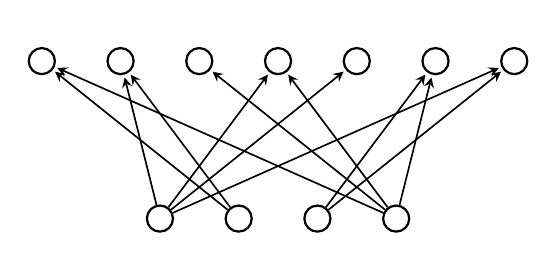
\begin{tikzpicture}[scale = 0.5,
            > = stealth, shorten > = 1pt, auto,
            semithick ]

        \tikzstyle{every state}=[
            draw = black,
            thick,
            minimum size = 1mm
        ]

        \node[state] at (0,0) (11) [label=below:] {};
        \node[state] at (2,0) (12)  [label=below:] {};
        \node[state] at (4,0) (21)  [label=below:] {};
        \node[state] at (6,0) (22)  [label=below:] {};
        \node[state] at (-3,4) (7)  [label=above:] {};
        \node[state] at (-1,4) (5)  [label=above:] {};
        \node[state] at (1,4) (4)  [label=above:] {};
        \node[state] at (3,4) (1)  [label=above:] {};
        \node[state] at (5,4) (3)  [label=above:] {};
\node[state] at (7,4) (2)  [label=above:] {};
        \node[state] at (9,4) (6)  [label=above:] {};

        \path[->] (11) edge  (5);
        \path[->] (11) edge  (1);
        \path[->] (11) edge  (3);
        \path[->] (11) edge  (6);
        
        \path[->] (12) edge  (7);
        \path[->] (12) edge  (5);
        
        \path[->] (21) edge  (2);
        \path[->] (21) edge  (6);
        
        \path[->] (22) edge  (2);
        \path[->] (22) edge  (1);
        \path[->] (22) edge  (4);
        \path[->] (22) edge  (7);
    \end{tikzpicture}
        }
  \caption{}
  \label{fig:enca}
\end{subfigure}
\hspace{4mm}
\begin{subfigure}{.31\textwidth}
  \centering
   \resizebox{\linewidth}{!}{
  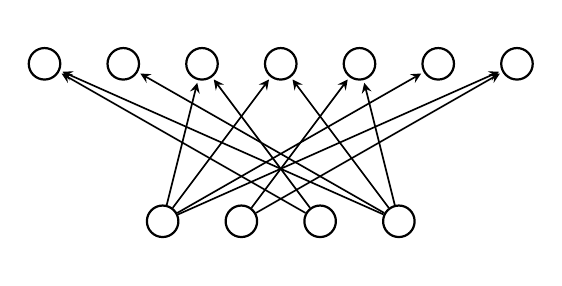
\begin{tikzpicture}[scale = 0.5,
            > = stealth, shorten > = 1pt, auto,
            node distance = 3cm, semithick ]

        \tikzstyle{every state}=[
            draw = black,
            thick,
            fill = white,
            minimum size = 4mm
        ]

        \node[state] at (0,0) (11) [label=below:] {};
        \node[state] at (2,0) (12)  [label=below:] {};
        \node[state] at (4,0) (21)  [label=below:] {};
        \node[state] at (6,0) (22)  [label=below:] {};
        \node[state] at (-3,4) (7)  [label=above:] {};
        \node[state] at (-1,4) (5)  [label=above:] {};
        \node[state] at (1,4) (4)  [label=above:] {};
        \node[state] at (3,4) (1)  [label=above:] {};
        \node[state] at (5,4) (3)  [label=above:] {};
        \node[state] at (7,4) (2)  [label=above:] {};
        \node[state] at (9,4) (6)  [label=above:] {};

        \path[->] (11) edge  (4);
        \path[->] (11) edge  (1);
        \path[->] (11) edge  (2);
        \path[->] (11) edge  (6);
        
        \path[->] (12) edge  (3);
        \path[->] (12) edge  (6);
        
        \path[->] (21) edge  (7);
        \path[->] (21) edge  (4);
        
        \path[->] (22) edge  (7);
        \path[->] (22) edge  (1);
        \path[->] (22) edge  (5);
        \path[->] (22) edge  (3);
    \end{tikzpicture}
    }
  \caption{}
  \label{fig:encb}
\end{subfigure}
\begin{subfigure}{.31\textwidth}
  \centering
     \resizebox{\linewidth}{!}{
  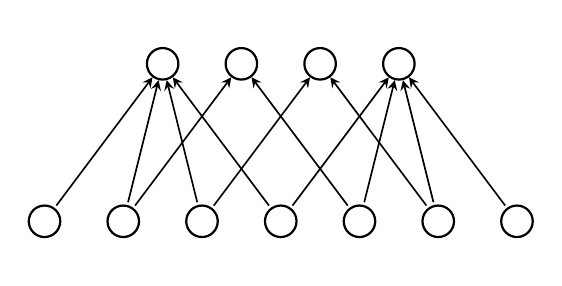
\begin{tikzpicture}[scale = 0.5,
            > = stealth, shorten > = 1pt, auto,
            node distance = 3cm, semithick ]

        \tikzstyle{every state}=[
            draw = black,
            thick,
            fill = white,
            minimum size = 4mm
        ]

        \node[state] at (0,4) (C11) [label=above:] {};
        \node[state] at (2,4) (C12)  [label=above:] {};
        \node[state] at (4,4) (C21)  [label=above:] {};
        \node[state] at (6,4) (C22)  [label=above:] {};
        \node[state] at (-3,0) (7)  [label=below:] {};
        \node[state] at (-1,0) (5)  [label=below:] {};
        \node[state] at (1,0) (4)  [label=below:] {};
        \node[state] at (3,0) (1)  [label=below:] {};
        \node[state] at (5,0) (3)  [label=below:] {};
        \node[state] at (7,0) (2)  [label=below:] {};
        \node[state] at (9,0) (6)  [label=below:] {};

        \path[<-] (C11) edge  (4);
        \path[<-] (C11) edge  (1);
        \path[<-] (C11) edge  (7);
        \path[<-] (C11) edge  (5);
        
        \path[<-] (C12) edge  (3);
        \path[<-] (C12) edge  (5);
        
        \path[<-] (C21) edge  (2);
        \path[<-] (C21) edge  (4);
        
        \path[<-] (C22) edge  (6);
        \path[<-] (C22) edge  (1);
        \path[<-] (C22) edge  (2);
        \path[<-] (C22) edge  (3);
    \end{tikzpicture}
    }
  \caption{}
  \label{fig:dec}
\end{subfigure}
\caption[Basic constructing blocks of Strassen's algorithm CDAG]{Basic constructing blocks of Strassen's CDAG. Note that  and  are isomorphic.}
\label{fig:fig}
\end{figure}
Let  denote the corresponding CDAG. For ,  can be obtained by using a recursive construction which mirrors the recursive structure of the algorithm. The base of the construction is the  CDAG which corresponds to the multiplication of two  matrices using Strassen's algorithm (Figure~\ref{fig:bsestra}).  can then be constructed by composing seven copies of , each corresponding to one of the seven sub-products generated by the algorithm (see Figure~\ref{fig:strarec}):  
   vertex-disjoint copies of CDAGs  (resp., ) are used to connect the input vertices of  which correspond to the values of the input matrix  (resp., ) to the appropriate input vertices of the seven sub-CDAGs ; the output vertices sub-CDAGs  (which  correspond to outputs of the seven sub-products) are connected to the opportune output vertices of the entire  CDAG  using  copies of the decoder sub-CDAG .
  
  \begin{figure}[bt]
  \begin{subfigure}{.48\textwidth}
  \centering
     \resizebox{\linewidth}{!}{
     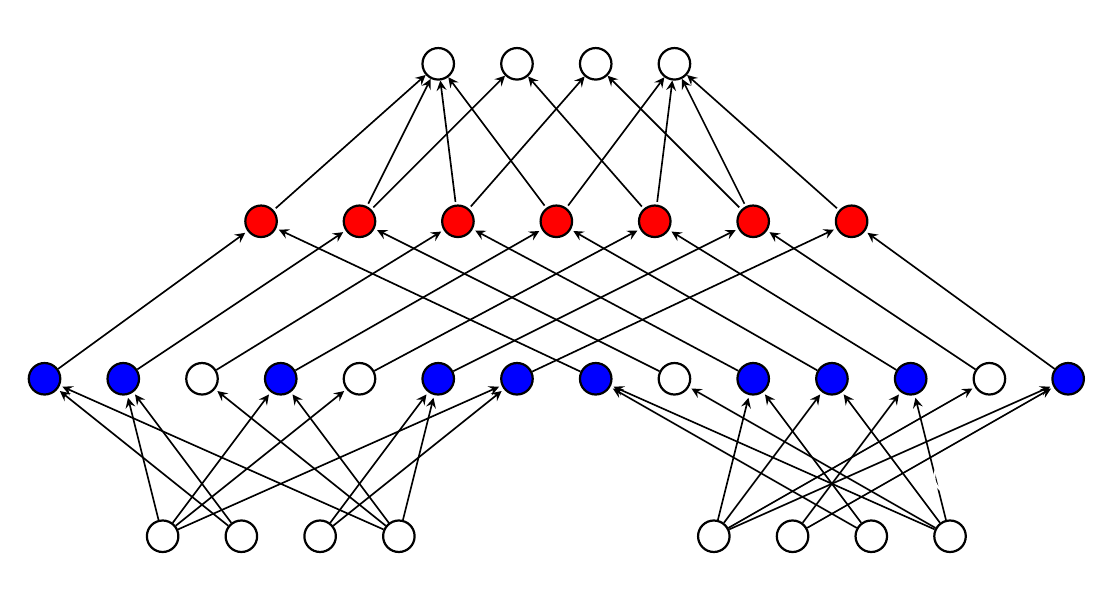
\begin{tikzpicture}[scale = 0.5,
            > = stealth, shorten > = 1pt, auto,
            node distance = 3cm, semithick ]

        \tikzstyle{every state}=[
            draw = black,
            thick,
            minimum size = 4mm
        ]
		\node[state] at (0,0) (A11) [label=below:] {};
        \node[state] at (2,0) (A12)  [label=below:] {};
        \node[state] at (4,0) (A21)  [label=below:] {};
        \node[state] at (6,0) (A22)  [label=below:] {};
        \node[state] at (-3,4) (A7)  [fill = blue] {};
        \node[state] at (-1,4) (A5)  [fill = blue] {};
        \node[state] at (1,4) (A4)    {};
        \node[state] at (3,4) (A1)   [fill = blue]{};
        \node[state] at (5,4) (A3)    {};
        \node[state] at (7,4) (A2)   [fill = blue] {};
        \node[state] at (9,4) (A6)   [fill = blue] {};

        \path[->] (A11) edge  (A5);
        \path[->] (A11) edge  (A1);
        \path[->] (A11) edge  (A3);
        \path[->] (A11) edge  (A6);
        
        \path[->] (A12) edge  (A7);
        \path[->] (A12) edge  (A5);
        
        \path[->] (A21) edge  (A2);
        \path[->] (A21) edge  (A6);
        
        \path[->] (A22) edge  (A2);
        \path[->] (A22) edge  (A1);
        \path[->] (A22) edge  (A4);
        \path[->] (A22) edge  (A7);
        
        \node[state] at (14,0) (B11) [label=below:] {};
        \node[state] at (16,0) (B12)  [label=below:] {};
        \node[state] at (18,0) (B21)  [label=below:] {};
        \node[state] at (20,0) (B22)  [label=below:] {};
        \node[state] at (11,4) (B7)  [fill = blue] {};
        \node[state] at (13,4) (B5)  {};
        \node[state] at (15,4) (B4)  [fill = blue] {};
        \node[state] at (17,4) (B1)  [fill = blue] {};
        \node[state] at (19,4) (B3)  [fill = blue] {};
        \node[state] at (21,4) (B2)   {};
        \node[state] at (23,4) (B6)  [fill = blue] {};

        \path[->] (B11) edge  (B4);
        \path[->] (B11) edge  (B1);
        \path[->] (B11) edge  (B2);
        \path[->] (B11) edge  (B6);
        
        \path[->] (B12) edge  (B3);
        \path[->] (B12) edge  (B6);
        
        \path[->] (B21) edge  (B7);
        \path[->] (B21) edge  (B4);
        
        \path[->] (B22) edge  (B7);
        \path[->] (B22) edge  (B1);
        \path[->] (B22) edge  (B5);
        \path[->] (B22) edge  (B3);

        \node[state] at (7,12) (C11) [label=above:] {};
        \node[state] at (9,12) (C12)  [label=above:] {};
        \node[state] at (11,12) (C21)  [label=above:] {};
        \node[state] at (13,12) (C22)  [label=above:] {};
        \node[state] at (2.5,8) (7)  [fill = red, label=left:] {};
        \node[state] at (5,8) (5)  [fill = red, label=left:] {};
        \node[state] at (7.5,8) (4)  [fill = red, label=left:] {};
        \node[state] at (10,8) (1)  [fill = red, label=left:] {};
        \node[state] at (12.5,8) (3)  [fill = red, label=left:] {};
        \node[state] at (15,8) (2)  [fill = red, label=left:] {};
        \node[state] at (17.5,8) (6)  [fill = red, label=left:] {};
        
        \node[state, draw= white] at (7,1.5) (ena)  [label=right: \LARGE ] {};
        \node[state, draw= white] at (20,1.5) (enb)  [label=right: \LARGE ] {};
        \node[state, draw= white] at (0,10.5) (dec)  [label=right: \LARGE] {};

        \path[<-] (C11) edge  (4);
        \path[<-] (C11) edge  (1);
        \path[<-] (C11) edge  (7);
        \path[<-] (C11) edge  (5);
        
        \path[<-] (C12) edge  (3);
        \path[<-] (C12) edge  (5);
        
        \path[<-] (C21) edge  (2);
        \path[<-] (C21) edge  (4);
        
        \path[<-] (C22) edge  (6);
        \path[<-] (C22) edge  (1);
        \path[<-] (C22) edge  (2);
        \path[<-] (C22) edge  (3);
        
        \path[->] (A7) edge  (7);
        \path[->] (B7) edge  (7);
        \path[->] (A5) edge  (5);
        \path[->] (B5) edge  (5);
        \path[->] (A4) edge  (4);
        \path[->] (B4) edge  (4);
        \path[->] (A1) edge  (1);
        \path[->] (B1) edge  (1);
        \path[->] (A3) edge  (3);
        \path[->] (B3) edge  (3);
        \path[->] (A2) edge  (2);
        \path[->] (B2) edge  (2);
        \path[->] (A6) edge  (6);
        \path[->] (B6) edge  (6);
    \end{tikzpicture}
     }
     \caption{Strassen's  CDAG}
     \label{fig:bsestra}
  \end{subfigure}	
  \hspace{1mm}
  \begin{subfigure}{.49\textwidth}
  \centering
     \resizebox{\linewidth}{!}{
     	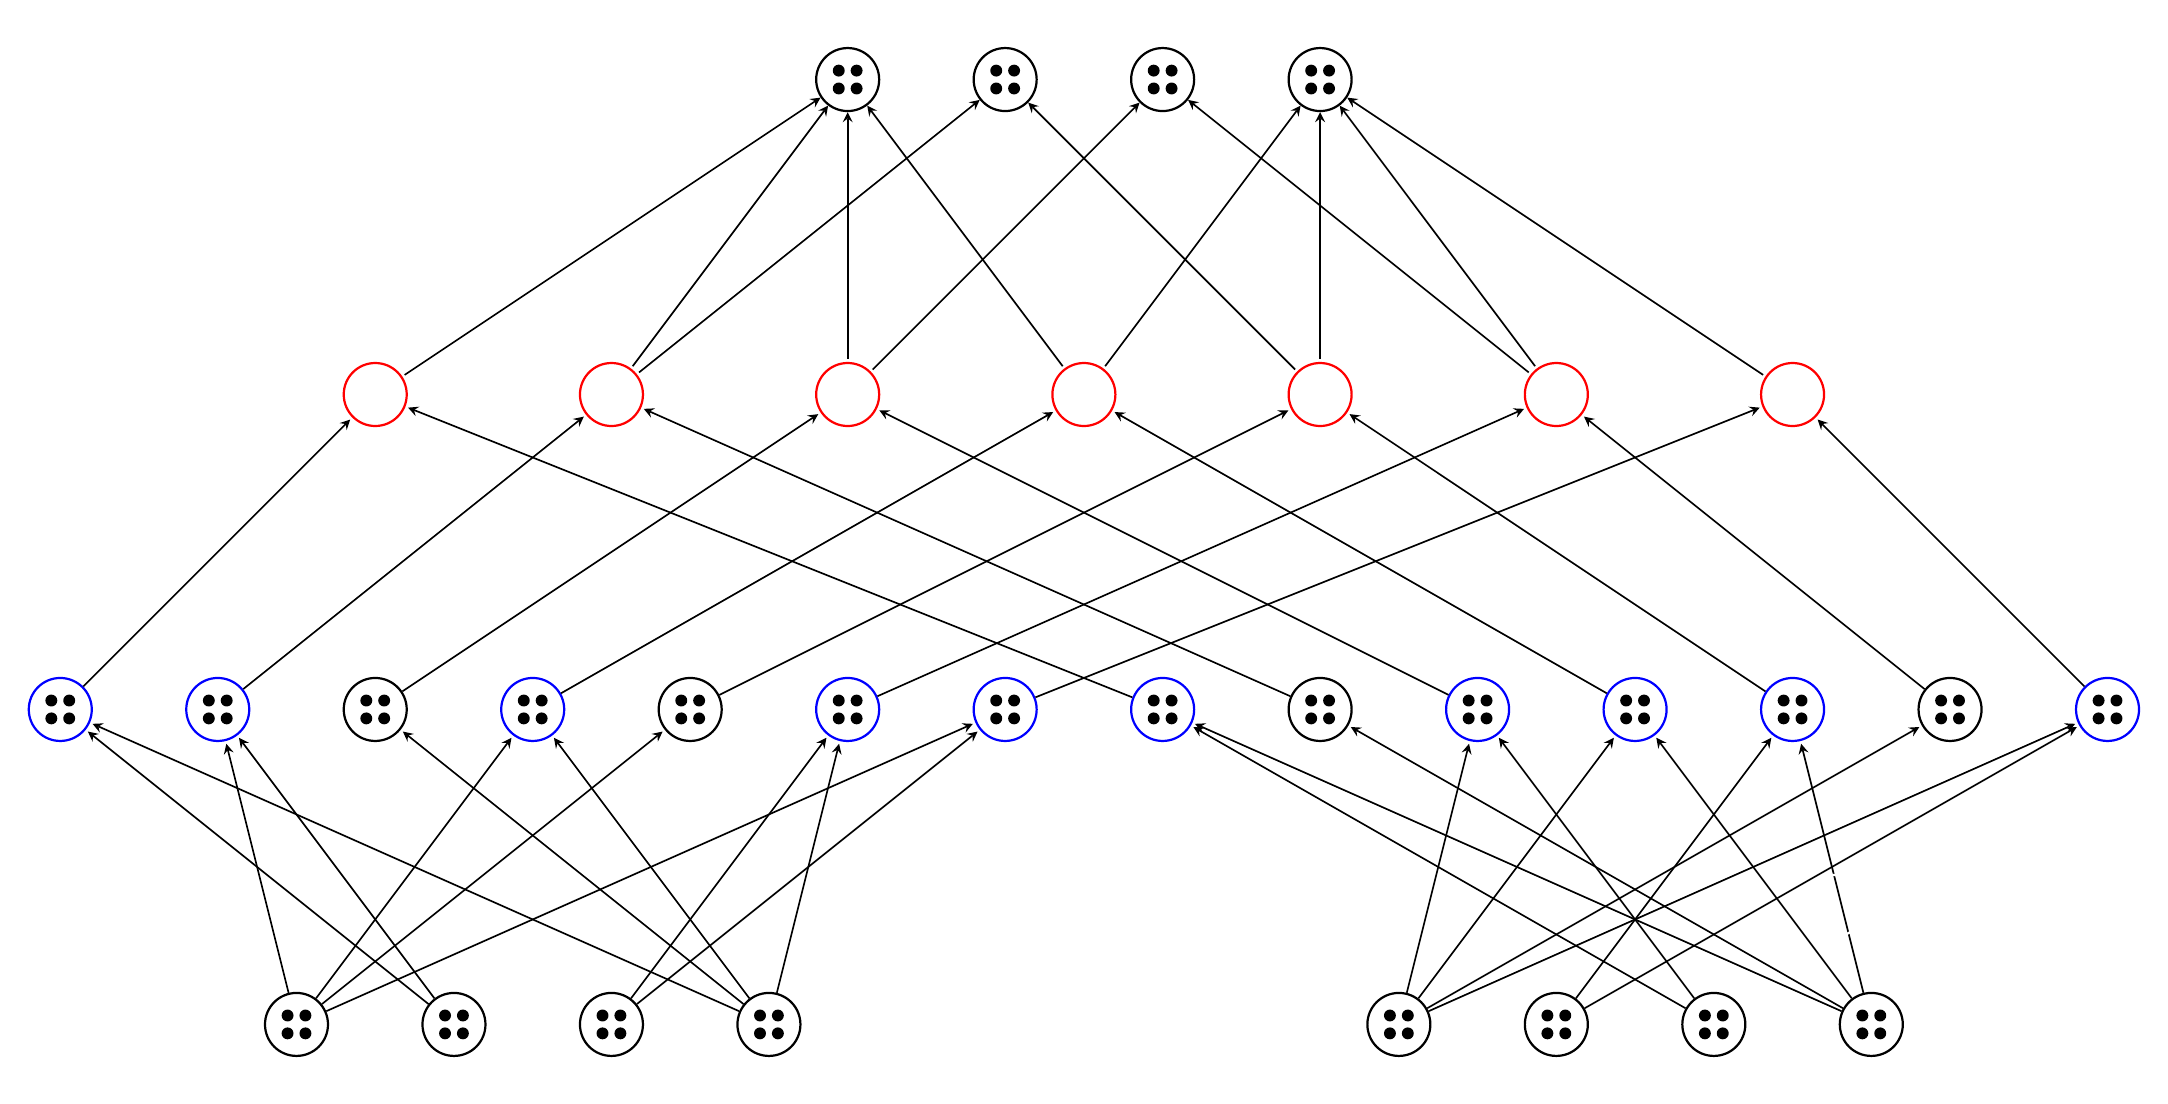
\begin{tikzpicture}[
            > = stealth, shorten > = 1pt, auto,
            node distance = 2cm, semithick ]

        \tikzstyle{every state}=[
            draw = black,
            thick,
            minimum size = 8mm
        ]
		\node[state, tokens=4] at (0,0) (A11) [label=below: \huge ] {};
        \node[state, tokens=4] at (2,0) (A12)  [label=below:\huge ] {};
        \node[state, tokens=4] at (4,0) (A21)  [label=below:\huge ] {};
        \node[state, tokens=4] at (6,0) (A22)  [label=below:\huge ] {};
        \node[state, draw = blue, tokens=4] at (-3,4) (A7)   {};
        \node[state, draw = blue, tokens=4] at (-1,4) (A5)   {};
        \node[state, tokens=4] at (1,4) (A4)    {};
        \node[state, draw = blue, tokens=4] at (3,4) (A1)    {};
        \node[state, tokens=4] at (5,4) (A3)    {};
        \node[state, draw = blue, tokens=4] at (7,4) (A2)    {};
        \node[state, draw = blue, tokens=4] at (9,4) (A6)    {};

        \path[->] (A11) edge  (A5);
        \path[->] (A11) edge  (A1);
        \path[->] (A11) edge  (A3);
        \path[->] (A11) edge  (A6);
        
        \path[->] (A12) edge  (A7);
        \path[->] (A12) edge  (A5);
        
        \path[->] (A21) edge  (A2);
        \path[->] (A21) edge  (A6);
        
        \path[->] (A22) edge  (A2);
        \path[->] (A22) edge  (A1);
        \path[->] (A22) edge  (A4);
        \path[->] (A22) edge  (A7);
        
        \node[state, tokens=4] at (14,0) (B11) [label=below:\huge ] {};
        \node[state, tokens=4] at (16,0) (B12)  [label=below:\huge ] {};
        \node[state, tokens=4] at (18,0) (B21)  [label=below:\huge ] {};
        \node[state, tokens=4] at (20,0) (B22)  [label=below:\huge ] {};
        \node[state, draw = blue, tokens=4] at (11,4) (B7)   {};
        \node[state, tokens=4] at (13,4) (B5)  {};
        \node[state, draw = blue, tokens=4] at (15,4) (B4)   {};
        \node[state, draw = blue, tokens=4] at (17,4) (B1)  {};
        \node[state, draw = blue, tokens=4] at (19,4) (B3)   {};
        \node[state, tokens=4] at (21,4) (B2)   {};
        \node[state, draw = blue, tokens=4] at (23,4) (B6)   {};

        \path[->] (B11) edge  (B4);
        \path[->] (B11) edge  (B1);
        \path[->] (B11) edge  (B2);
        \path[->] (B11) edge  (B6);
        
        \path[->] (B12) edge  (B3);
        \path[->] (B12) edge  (B6);
        
        \path[->] (B21) edge  (B7);
        \path[->] (B21) edge  (B4);
        
        \path[->] (B22) edge  (B7);
        \path[->] (B22) edge  (B1);
        \path[->] (B22) edge  (B5);
        \path[->] (B22) edge  (B3);

        \node[state, tokens=4] at (7,12) (C11) [label=above:\huge ] {};
        \node[state, tokens=4] at (9,12) (C12)  [label=above:\huge ] {};
        \node[state, tokens=4] at (11,12) (C21)  [label=above:\huge ] {};
        \node[state, tokens=4] at (13,12) (C22)  [label=above:\huge ] {};
        \node[state, draw = red] at (1,8) (7)  {\huge };
        \node[state, draw = red] at (4,8) (5)  {\huge };
        \node[state, draw = red] at (7,8) (4)  {\huge};
        \node[state, draw = red] at (10,8) (1)  {\huge };
        \node[state, draw = red] at (13,8) (3) {\huge };
        \node[state, draw = red] at (16,8) (2)  {\huge };
        \node[state, draw = red] at (19,8) (6)  {\huge };
        
        \node[state, draw= white] at (7,1.5) (ena)  [label=right: \Huge ] {};
        \node[state, draw= white] at (19.5,1.5) (enb)  [label=right: \Huge ] {};
        \node[state, draw= white] at (-1,10.5) (dec)  [label=right:\Huge ] {};

        \path[<-] (C11) edge  (4);
        \path[<-] (C11) edge  (1);
        \path[<-] (C11) edge  (7);
        \path[<-] (C11) edge  (5);
        
        \path[<-] (C12) edge  (3);
        \path[<-] (C12) edge  (5);
        
        \path[<-] (C21) edge  (2);
        \path[<-] (C21) edge  (4);
        
        \path[<-] (C22) edge  (6);
        \path[<-] (C22) edge  (1);
        \path[<-] (C22) edge  (2);
        \path[<-] (C22) edge  (3);
        
        \path[->] (A7) edge  (7);
        \path[->] (B7) edge  (7);
        \path[->] (A5) edge  (5);
        \path[->] (B5) edge  (5);
        \path[->] (A4) edge  (4);
        \path[->] (B4) edge  (4);
        \path[->] (A1) edge  (1);
        \path[->] (B1) edge  (1);
        \path[->] (A3) edge  (3);
        \path[->] (B3) edge  (3);
        \path[->] (A2) edge  (2);
        \path[->] (B2) edge  (2);
        \path[->] (A6) edge  (6);
        \path[->] (B6) edge  (6);
    \end{tikzpicture}
     }
     \caption{Recursive construction of the  CDAG}
     \label{fig:strarec}
  \end{subfigure}

  \caption{Blue vertices represent combinations of the input values from the factor matrices  and  which are used as input values for the sub-problems ; red vertices represent the output of the seven sub-problems which are used to compute the output values of the product matrix .}
\end{figure} 

In our proofs we will leverage the following two properties of Strassen's CDAG:
\begin{lemma}\label{lem:disictness_sub_cdag}
Let   denote the CDAG of Strassen's algorithm for input matrices of size . For , there are exactly  sub-CDAGs  which do not share any vertex in  (i.e., they are \emph{vertex disjoint sub-CDAGs of }).
\end{lemma}
\begin{lemma}\label{lem:conneconder}
Given an encoder CDAG, for any subset  of its output vertices, there exists a sub-set  of its input vertices such that each vertex in  can be connected to a distinct vertex in  where .
\end{lemma}

The validity of this lemmas can be verified through an analysis of respectively, the recursive structure of Strassen's CDAG and the properties of  the encoding sub-CDAGs  and . We refer the reader to Appendix~\ref{app:proof_encoder} for detailed proofs.

\paragraph*{Strassen-like algorithms}
A -Strassen-like algorithm has a recursive structure for
which in the ``\emph{base case}'' two  matrices are
multiplied using  scalar multiplications, whose result are then
combined to obtain the product matrix.  Given input matrices of size
, the algorithm splits them into  sub-matrices of
size  and then proceeds block-wise, according to
the base case. Additions (resp., subtractions) in the base case are
interpreted as additions (resp., subtractions) of blocks and are
performed element-wise. Multiplications in the base case are
interpreted as multiplications of blocks and are executed by
recursively calling the algorithm. In our analysis we consider
Strassen-like algorithms for which each linear combination of the
input sub-matrices is used in only one multiplication.

Let  be the CDAG corresponding to a -Strassen-like algorithm for input matrices of size
 .  has a recursive structure analogous
to that of Strassen's CDAG . The base element
 of the CDAG construction corresponding to the
base case consists of two \emph{encoding graphs} (corresponding
respectively to the sub-CDAGs  and  for ), which compute  linear combinations of entries of
respectively the factor matrix  and of . Corresponding pairs are
then multiplied and the outputs are then combined using an
\emph{decoder} sub-CDAG to obtain the output.

Although in general the sub-problems generated by a Strassen-like
algorithm may not be input disjoint, in~\cite{scott2015matrix} Scott
et al. showed that a property similar to
Lemma~\ref{lem:disictness_sub_cdag} holds:

\begin{lemma}[Lemma 1~\cite{scott2015matrix}]\label{lem:vdigraphslike}
Let  denote the CDAG of a
-Strassen-like algorithm for input matrices of size . For , there are at least
 vertex-disjoint sub-CDAGs 
in .
\end{lemma}
For completeness, we summarize their result in
Appendix~\ref{app:proof_encoder}.

\section{Lower bounds for schedules without recomputation}\label{sect:stranore}
In our presentation we denote as  the CDAG corresponding to the execution of an \emph{unspecified} algorithm which implements the square matrix multiplication function . 
Let  be a CDAG composed by  vertex-disjoint CDAGs
. The set  (resp., ) of input (resp., output)
vertices of  is given by the union of the sets of the
input (resp., output) vertices of the  sub-CDAGs . According to this definition, the CDAG of Strassen  is a  CDAG for
 (Lemma~\ref{lem:disictness_sub_cdag}). 

\begin{lemma}\label{lem:newbasenr}
Given , let  be a subset of its the output
vertices. For any subset  of the vertices of 
with , the set  of the input
vertices which are not post-dominated by  satisfies .
\end{lemma}
\begin{proof}
	Let  (resp., ) denote the subset of  (resp., ) which correspond to vertices in the -th sub CDAG  for . As, by hypothesis, the sub-CDAGs  are vertex disjoint,  (resp., ) constitute a partition of  (resp., ). 
	
	Let  denote the set of input vertices of  for which  is a post-dominator with respect to . 
From Lemma~\ref{lem:info_flo_mat_mul} and Lemma~\ref{lem:flowpost} the following condition must hold:
		
	Let  denote the set of input vertices of  for which  is a post-dominator with respect to . Since , from (\ref{eq:newlem1}) we have .
	
	As the sub-CDAGs  are vertex disjoint, we can state that all the vertices in  are not post-dominated by  and
	.
\end{proof}

\begin{corollary}\label{cor:domnr}
	Given , the minimum size of a dominator set of any subset of the output vertices  is at least .	
\end{corollary}

These results allows us to obtain a general theorem on the \io
complexity of matrix multiplication algorithms under the no-recomputation assumption.

\begin{theorem}[Lower bound \io complexity  matrix multiplication with no recomputation]
\label{thm:strassnr}
Let   the CDAG corresponding to an algorithm  which computes the product of two square matrices . Suppose that   has  vertex disjoint sub-CDAGs  each of which corresponds to input-disjoint sub-products of matrices of size  generated by . 
Assuming no intermediate result is ever computed more than once, the \io-complexity of  when run on a sequential machine with a cache of size  is:

If run on  processor each equipped with a local memory of size M the \io complexity is:

\end{theorem}
\begin{proof}
	As first observation, note that the  vertex-disjoint sub-CDAGs  constitute a  CDAG as previously defined. The set  of input (resp.  of output) vertices of  is composed by the union of the input (resp., output) vertices of the  sub-CDAGs . Clearly, .
	
	We start by proving (\ref{eq:seqnewnr}). Let  be any computational schedule for the sequential execution of the algorithm  using a cache of size  for which each intermediate value is computed just once. Each intermediate value must therefore be kept in memory (either cache or slow) until all operations using it as an operand have been computed. The operations corresponding to vertices in  are executed according to a topological ordering of the vertices, that is, any value corresponding to a vertex in  which can be connected through a directed path to a vertex in  will be computed in  before . We partition  into  segments such that during each segment  the values corresponding to exactly  vertices in  (denoted as ) are computed for the first (and only) time.	
	We shall now verify that at least  \io operations are to be executed during every segment . The proof is by contradiction.   
	 Let  denote the set of vertices of  which correspond to the at most  values which are  stored in the cache at the beginning of the segment and the at most  values which are loaded into the cache form the slow memory during  by means of a \emph{read} \io operation. We thus have .
	  In order for the  values corresponding to vertices in  to be computed during the segment without any additional \io operation, there must be no path connecting any vertex in  to any vertex in  which does not have at least one vertex in  (i.e.  has to be a \emph{dominator set} of ). If any such path exists then there is a previously computed intermediate result  which is required for the computation of at lest one of the values corresponding to a vertex in  which is neither residing in the cache at the beginning of , nor loaded from slow memory to the cache. As no intermediate result can be computed twice this would lead to a contradiction.  From Corollary~\ref{cor:domnr}, we have that any sub-set of  elements of  has dominator size at least . This leads to a contradiction.
	
	At least  \io operations are thus executed during each segment . Since, by construction, the  segments are not overlapping, we can conclude that at least  \io operations are necessary for the execution of . This concludes the proof for lower bound in (\ref{eq:seqnewnr}).
	
	The proof for the lower bound for the parallel model in equation (\ref{eq:parnewnr}), follows a similar strategy. If  processors are being used, at least one such processor  must compute at least  values corresponding to vertices in . The bound follows by applying the same argument discussed for the sequential case to the computation executed by .
	\end{proof}

This general result can be steadily applied to Strassen-like algorithms.
\begin{corollary}
Consider Strassen's algorithm being used to multiply two square
matrices .  Assuming no intermediate result is
ever computed more than once, the I/O-complexity of the algorithm run
on a sequential machine with a cache of size  is:

If run on  processor each equipped with local memory of size  the \io complexity is:

Additionally, the I/O-complexity of any -Strassen-like algorithm run on a sequential machine with a cache of size  is:

If run on  processor each equipped with local memory of size  the \io complexity is:

\end{corollary}
\begin{proof}
	We provide a simple proof for the sequential cases in (\ref{eq:stranr}) and (\ref{eq:stranrlike}). Let us assume without loss of generality that  and   for some . At least  \io operations are necessary in order to read all the  input values form slow memory to the cache and to write the  output values to the slow memory once they have been computed. The statement of the theorem is therefore trivially verified if . 
For , the result in (\ref{eq:stranr}) follows from applying Theorem~\ref{thm:strassnr} to the  CDAG which, from Lemma~\ref{lem:disictness_sub_cdag}, has  vertex-disjoint sub CDAGs . 
The result in (\ref{eq:stranrlike}) similarly follows from applying Lemma~\ref{lem:vdigraphslike}. The results for the parallel model in (\ref{eq:stranrpar}) and (\ref{eq:stranrlikepar}) can be obtained using a generalization similar to the one described in Theorem~\ref{thm:strassnr}.
\end{proof}
While our lower bounds correspond asymptotically to the known bounds
in~\cite{scott2015matrix}, our technique yields a simpler analysis,
especially for the \io complexity of Strassen-like algorithms. Our
proof technique is based on the analysis of the recursive structure of
Strassen-like algorithms and on the identification of the
vertex-disjoint sub-CDAGs corresponding to the various
sub-problems. The fact that Theorem~\ref{thm:strassnr} applies for
\emph{any} square matrix multiplication algorithm, allows us to obtain
significant bounds without a detailed analysis of the CDAG
corresponding to the \emph{specific} algorithm being considered.

This property further suggests that our technique may be amenable to
deal with hybrid ``\emph{non-stationary}'' multiplication algorithms, which allow mixing of schemes of the previous Strassen-like class in different recursive levels (for the ``\emph{uniform}'' sub-class)~\cite{douglas1994gemmw}, or even within the same level (for the ``\emph{non-uniform}'' sub-class).

\section{Lower bounds for schedules with recomputation}\label{sec:stragen}
Under no-recomputation assumption once an input value is loaded in memory or an intermediate result is calculated it is then necessary to maintain it in memory (either cache or slow) until the result of each operation which uses it as an input argument has been evaluated. This constitutes the foundation of the lower bound technique discussed in Theorem~\ref{thm:strassnr} as well as several other techniques discussed in literature (among others, the ``\emph{dichotomy width} technique''~\cite{bilardi1999processor}, the ``\emph{boundary flow} technique''~\cite{ranjan2012upper}), including those yielding \io lower bound for Strassen's algorithm~\cite{ballard2012graphrec,scott2015matrix}. If recomputation is allowed, intermediate results can instead be deleted from \emph{all} memory and recomputed. This introduces a substantial complication in the theoretical analysis of the \io cost (see~\cite{ballard2011minimizing} for an extensive discussion). \\

In this section we present a new lower bound technique which yields a novel asymptotically tight \io lower bound for Strassen's algorithm both in the sequential and parallel model.
We start by presenting some technical lemmas which  will then be used for the proof of our main result in Theorem~\ref{thm:genstrass}. 

\begin{lemma}\label{lem:stra_part1}
Let  be the CDAG which corresponds to the execution of Strassen's matrix multiplication algorithm for input matrices , with . Let  (resp., ) denote the set of input (resp., output) vertices of the  sub-CDAGs . Furthermore, let  be a subset of the set of \emph{internal} (i.e., not input) vertices of the sub-CDAGs . Let  denote the set on input vertices of . For any subset  such that  there exists a set  with  such that  vertices in  can be connected to vertices in a subset , with  via vertex disjoint paths. Furthermore all vertices in  can be connected to a vertex in  by a directed path which does not include any vertex in .
\end{lemma}
\begin{proof}
	The proof is by induction on the size of the input matrices.\\
\emph{Base:} In the base case we have . We therefore
have  and the sets
 and  coincide. We can verify that the
statement holds by simply applying Lemma~\ref{lem:newbasenr} as
 corresponds to a  CDAG.\\
\emph{Inductive step:} Let us now assume that the statement is
verified for , with . We shall show
that the statement is verified for  as well.  Let
 denote the
seven sub-CDAGs of , each corresponding to one of the
seven sub-products generated by the first recursive step of Strassen's
algorithm. Let  (resp., ) denote the subset of 
(resp., ) which correspond to vertices in . As, from Lemma~\ref{lem:disictness_sub_cdag}, the seven
sub-CDAGs  are vertex disjoint among themselves,
 (resp., ) constitute a partition of  (resp., ).

For , let  be the subset of vertices in  in the sub-CDAGs . Again, as the seven sub-CDAGs  are vertex disjoint among themselves, we have that  is a partition of .  This implies . Let , we have . 
	
	Applying the inductive hypothesis to each sub-CDAG , we have that there is a subset  with  such that vertices of  are connected  to vertices in  via paths which do not include any vertex in . Furthermore vertices in  can be connected to a subset  of the input vertices of  with , using vertex-disjoint paths. Since the sub-CDAGs  are vertex disjoint, so are the paths connecting vertices in  to vertices in . In order to conclude our proof we need to show that is possible to extend at least  of these paths to vertices in  while still being vertex disjoint. 
	
	According to the construction of Strassen's CDAG, vertices in   are connected to vertices in  by means of  encoding sub-CDAGs  and  ( of each). For the construction of , none of these encoding sub-CDAGs shares any input or output vertices. For any given encoder sub-CDAGs each of its output vertices belongs to a different sub-CDAG . This fact ensures that for a single sub-CDAG  it is possible to connect all the vertices in  to a subset of the vertices in  via vertex disjoint paths.
	
	For each of the  encoder sub-CDAGs, let us consider the vector . We have that  if the corresponding -th output vertex (respectively according to the numbering indicated in Figure~\ref{fig:enca} or Figure~\ref{fig:encb}) is in  or  otherwise. We therefore have that  corresponds to the number of output vertices of the -th encoder sub-CDAG which are in .
	 From Lemma~\ref{lem:conneconder}, we have that for each encoder sub-CDAG there exists a subset  of the input vertices of the -th encoder sub-CDAG for which is possible to connect each vertex in  to a distinct output vertex of the -th encoder sub-CDAG using vertex disjoint paths, each constituted by a singular edge with . The number of vertex disjoint paths connecting vertices in , to vertices in  is therefore at least , under the constraint that .
		Without loss of generality, let us assume that . As previously stated, it is possible to connect all vertices in  to vertices in  through vertex disjoint paths. Consider now all possible dispositions of the vertices in  over the outputs of the  encoder sub-CDAGs. 
		Recall that the output vertices of an encoder sub-CDAG belong each to a different  sub-CDAG. From Lemma~\ref{lem:conneconder}, we have that for each encoder, there exists a subset  of the input vertices of the -th encoder sub-CDAG, with
		, 		for which is possible to connect all vertices in  to  \emph{distinct} output vertices of the -th encoder sub-CDAG which are in  using , thus using vertex disjoint paths.
As all the  sub-CDAGs are vertex disjoint, we can sum their contributions and we can therefore conclude that the number of vertex disjoint paths connecting values in  to vertices in   is at least .
	Squaring this quantity leads to:
	
	As, by assumption, , we have:  for . Thus:
	
	
	There are therefore at least  vertex disjoint paths connecting vertices in  to vertices in . The lemma follows.
\end{proof}

\begin{lemma}\label{lem:stra_part2}
Let  be the CDAG which corresponds to the execution of Strassen's matrix multiplication algorithm for input matrices , with . Let  (resp., ) denote the set of input (resp., output) vertices of the  sub-CDAGs . Any dominator set for any subset , has size at least .
\end{lemma}
\begin{proof}
	The proof is by contradiction. Let  be a dominator set for  in  such that . 
	Let  be the subset of ``internal'' vertices of any of any of the sub-CDAGs  in .	Let  denote the set the input vertices of . From Lemma~\ref{lem:stra_part1} we have that there exist at least   paths connecting a subset  of global input vertices to vertices in  which do not include any vertex in . Further, the sub-paths of such paths that connect vertices in  to vertices in  are vertex disjoint among themselves. This implies that each of the vertices in   can therefore be traversed by at most one of these paths. The number of directed paths from  to  which do not traverse any vertex in  will therefore be at least . We have:

Since by hypothesis , we have ,
and thus .

For  there is therefore at least one path connecting an input vertex to a vertex in  which does not traverse any vertex in . This constitutes a contradiction.
\end{proof}

Lemma~\ref{lem:stra_part2} provides us with the tools required to obtain our main result. 

\begin{theorem}[Lower bound \io complexity Strassen's algorithm]
\label{thm:genstrass}
Consider Strassen's algorithm being used to multiply two square matrices . 
The I/O-complexity of Strassen's algorithm when run on a sequential machine with a cache of size  is:

If run on  processors each equipped with a local memory of size  the \io complexity is:

\end{theorem}
\begin{proof}
We start by proving (\ref{eq:seqnewnr}). We assume without loss of generality that  and   for some . At least  \io operations are necessary in order to read all the  input values form slow memory to the cache and to write the  output values to the slow memory once they have been computed. The theorem is therefore verified if . 

For , let  denote the set of output vertices of the  sub-CDAGs  of .
	Let  be any computation schedule for the sequential execution of Strassen's algorithm using a cache memory of size . 
	We partition  into segments such that during each segment  the values corresponding to exactly  distinct vertices in  (denoted as ) are computed for the \emph{first time}. As we have , there will be  such segments.
We shall now verify that at least  \io operations are to be executed during every segment . The proof is by contradiction.   
	 Let  denote the set of vertices of  which correspond to the at most  values which are stored in the cache at the beginning of the -th segment and to the at most  values loaded into the cache form the slow memory during  by means of a \emph{read} \io operation. We then have .
	 In order for the  values from  to be computed during the segment without any additional \io operation, there must be no path connecting any vertex in  to any input vertex of  which does not have at least one vertex in  (i.e.  has to be a \emph{dominator set} of ). From Lemma~\ref{lem:stra_part2}, we have that any sub-set of  elements of  has dominator size at least . This leads to a contradiction.
	
	At least  \io operations are thus executed during each segment . Since, by construction, the  segments are not overlapping, we can therefore conclude that at least  \io operations are necessary for the execution of any computation schedule . This concludes the proof for lower bound for the sequential case in (\ref{eq:stramain}). \\
	The proof for the bound for the parallel model in equation (\ref{eq:strapar}), follows a similar strategy: at least one of the  processors being used, denoted as , must compute at least  values corresponding to vertices in . The bound follows by applying the same argument discussed for the sequential case to the computation executed by . 
	\end{proof}

In~\cite{ballard2012communicationalg}, Ballard et al. presented a version of Strassen's algorithm whose \io cost matches, up to a constant the lower bound obtained in Theorem~\ref{thm:genstrass}. This implies that our bound is indeed asymptotically tight and that  the version of Strassen's algorithm presented by Ballard et al. in~\cite{ballard2012communicationalg}, is indeed asymptotically optimal with respect to the \io cost. Furthermore, as in the optimal algorithm presented in~\cite{ballard2012communicationalg} no intermediate result is ever recomputed, we can conclude the use of recomputation can lead at most to a constant factor reduction of the \io complexity for the execution of Strassen's matrix multiplication algorithm. 
	
\section{Conclusions}\label{sec:conlcusion}

This work has contributed to the characterization of the \io
complexity of Strassen's algorithm, by establishing asymptotically
tight lower bounds that hold even when recomputation is allowed.
The technique we have developed crucially exploits the recursive
nature of the CDAG, which makes it promising for the analysis of other
recursive algorithms, beginning with fast rectangular matrix
multiplication algorithms~\cite{le2012faster}.

The relationship we have exploited between dominator size and
Grigoriev's flow points at connections between \io complexity,
(pebbling) space-time tradeoffs~\cite{savage97models}, and VLSI
area-time tradeoffs~\cite{thompson79vlsistoc}; these connections
deserve further attention.

Some CDAGs for which non trivial \io complexity lower bounds are known
only in the case of no recomputations are described
in~\cite{bilardi1999processor}. These CDAGs are of particular interest
as examples of speedups superlinear with the number of processors, in
the ``\emph{limiting technology}'', defined by fundamental limitations on
device size and message speed.  Whether such speedups hold even when
recomputation is allowed remains an open question, which the
techniques introduced here might help answer.

In general, while it is well known that recomputation may reduce the
\io complexity of some CDAGs, we are far from a characterization of
those CDAGs for which recomputation is effective. This broad goal
remains a challenge for any attempt toward a general theory of the
communication requirements of computations.
\subparagraph*{Acknowledgements.}

This work was supported, in part, by MIUR of Italy under project
AMANDA 2012C4E3KT 004 and by the University of Padova under projects
STPD08JA32, CPDA121378/12, and CPDA152255/15.





\bibliography{bibliography}
\clearpage

\appendix
\section{Properties of Strassen's algorithm}

\begin{algorithm}
\caption{Strassen's Matrix Multiplication}\label{alg:strass}
\begin{algorithmic}[1]
	\Statex \textbf{Input:} matrices 
	\Statex \textbf{Output:} matrix 
	\Procedure{StrassenMM}{A,B}
	\If{}
	\State 
	\Else
	\State Decompose  and  into four equally sized bloc matrices as follows:
	\Statex 
\State 
\State 
\State 
\State 
\State 
\State 
\State 
\State  
\State 
\State 
\State 
\EndIf
\Return 
\EndProcedure
\end{algorithmic}
\end{algorithm}

The original version of  Strassen's fast matrix multiplication~\cite{strassen1969gaussian} is reported in Algortihm~\ref{alg:strass}. We refer the reader to~\cite{winograd1971multiplication} for
Winograd's variant, which reduces the number of additions. 

\label{app:proof_encoder}
\begin{proof}[Proof of Lemma~\ref{lem:disictness_sub_cdag}]
	Let us consider a single recursive step. While some of the sub-problems may use as input values form either  and  without any combination (i.e.,  uses the sub-matrix  as input), none of the seven sub-problems share any of their input values. As this consideration holds for each level of the recursive construction, we have that the  sub-problems with input of size  generated by of Strassen's algorithm do not share any input value.
\end{proof}

\begin{proof}[Proof of Lemma~\ref{lem:conneconder}]
We provide the proof for , as  and  are isomorphic,  the result holds for  as well. 
	Note that in  there are some pairs of input-output vertices  for which the input vertex  is the only predecessor of the output vertex . This implies that the two vertices are actually one unique vertex. With a little abuse of notation, we will still say that   can be connected to  via a single edge.
		
	We assign an index to each of the output vertices of  according to how is indicated in Figure~\ref{fig:enca}.  
Note that the index assigned to each output corresponds to the index of the sub-problem generated by Strassen's algorithm for which the corresponding value is used as an input (see Figure~\ref{fig:bsestra} and Figure~\ref{fig:strarec} in Section~\ref{sec:preliminaries}). 

In order to verify that this lemma holds, we study all possible compositions of a subset  of the output vertices of .  Each of these compositions is identified by a vector  with seven components, where  if the -th output of  is in  or zero otherwise, for . In order to improve the presentation, we associate to each of the possible 128 compositions a \emph{code} given by . In Table~\ref{table:configurations}, we study each of the 128 possible compositions of , which are ordered by the value of  and by their code. The value in the last column  denotes the maximum size of a sub-set  of the input vertices of  such that each vertex in  can be connected to a distinct vertex in the subset  corresponding to . Each of these values can be obtained through a straightforward analysis of .
The lemma then follows from observing that for any possible composition of the set  we have

\end{proof}

\begin{proof}[Proof of Lemma~\ref{lem:vdigraphslike}]
A proof for this result was presented in~\cite{scott2015matrix} (Lemma 1). For completeness, we present here a version of the proof using our notation.

Given an -Strassen like algorithm used to multiply , let  denote the corresponding CDAG. The recursive structure of the algorithm will generate a total of  sub-problems with input size  each of which corresponds to a sub-CDAGs .

The lemma is trivially verified for , in the following we consider the case for . As by hypothesis, non-trivial combinations of the input matrices are used as input for at most one sub-problem, the only input values which two sub-problems of the same size  can  share are sub-matrices of the ``\emph{global}'' input matrices . For , et  be one of the sub-computations corresponding to one of the sub-CDAGs  which multiplies matrices  and . 
Without loss of generality we assume that for both the basic encoder CDAGs for  and  at least one of the outputs is given by a non-trivial linear combination of elements of the input matrix. It is in fact well known that any algorithm which computes linear combinations of only one of the input matrices performs no better than the na\'ive-definition based matrix multiplication and it is therefore not a Strassen-like fast matrix multiplication algorithm.
This implies that at least one of the sub-problems  generated by  multiplies matrices  and  such that  is a nontrivial linear combination of sub-matrices of . Similarly, at least one of the  sub-computations  generated by  multiplies matrices  by  such that  is  non-trivial linear combination of sub-matrices of .  (resp., ) shares no input with  (resp., B). Thus at least one of the  sub-computations for input size   generated by  is input-disjoint from it. 
As by hypothesis, non-trivial combinations of the input matrices are used as input for at most one sub-problem, all the sub-computations  corresponding to each  are input-disjoint and the corresponding sub-CDAGs  are thus vertex disjoint.
\end{proof}
	\begin{longtable}[c]{|p{.04\textwidth}||p{.02\textwidth}||p{.03\textwidth} p{.03\textwidth} p{.03\textwidth} p{.03\textwidth} p{.03\textwidth} p{.03\textwidth} p{.03\textwidth}|p{.02\textwidth}|}
		\caption{Study of the possible compositions of sub-sets of output vertices of  for Lemma~\ref{lem:conneconder}}\label{table:configurations}\\ 
		\hline
		code &  &  &  &  &  &  &  &  &   \\\hline
		\endfirsthead
		\hline
		\multicolumn{10}{|c|}{{Table~\ref{table:configurations} - continued from previous page}}\\\hline
		code &  &  &  &  &  &  &  &  &  \\\hline
		\endhead
		
		\hline
		\multicolumn{10}{|c|}{{Continued on next page}}\\\hline
		\endfoot	
		
\hline 
\endlastfoot
			0   & 0 & 0 & 0 & 0 & 0 & 0 & 0 & 0 & 0 \\\hline
			1   & 1 & 0 & 0 & 0 & 0 & 0 & 0 & 1 & 1 \\
			2   & 1 & 0 & 0 & 0 & 0 & 0 & 1 & 0 & 1 \\
			4   & 1 & 0 & 0 & 0 & 0 & 1 & 0 & 0 & 1 \\
			8   & 1 & 0 & 0 & 0 & 1 & 0 & 0 & 0 & 1 \\
			16  & 1 & 0 & 0 & 1 & 0 & 0 & 0 & 0 & 1 \\
			32  & 1 & 0 & 1 & 0 & 0 & 0 & 0 & 0 & 1 \\
			64  & 1 & 1 & 0 & 0 & 0 & 0 & 0 & 0 & 1 \\\hline
			3   & 2 & 0 & 0 & 0 & 0 & 0 & 1 & 1 & 2 \\
			5   & 2 & 0 & 0 & 0 & 0 & 1 & 0 & 1 & 2 \\
			6   & 2 & 0 & 0 & 0 & 0 & 1 & 1 & 0 & 2 \\
			9   & 2 & 0 & 0 & 0 & 1 & 0 & 0 & 1 & 2 \\
			10  & 2 & 0 & 0 & 0 & 1 & 0 & 1 & 0 & 2 \\
			12  & 2 & 0 & 0 & 0 & 1 & 1 & 0 & 0 & 2 \\
			17  & 2 & 0 & 0 & 1 & 0 & 0 & 0 & 1 & 2 \\
			18 	& 2 & 0 & 0 & 1 & 0 & 0 & 1 & 0 & 2 \\
			20  & 2 & 0 & 0 & 1 & 0 & 1 & 0 & 0 & 2 \\
			24  & 2 & 0 & 0 & 1 & 1 & 0 & 0 & 0 & 2 \\
			33  & 2 & 0 & 1 & 0 & 0 & 0 & 0 & 1 & 2 \\
			34  & 2 & 0 & 1 & 0 & 0 & 0 & 1 & 0 & 2 \\
			36  & 2 & 0 & 1 & 0 & 0 & 1 & 0 & 0 & 2 \\
			40  & 2 & 0 & 1 & 0 & 1 & 0 & 0 & 0 & 2 \\
			48  & 2 & 0 & 1 & 1 & 0 & 0 & 0 & 0 & 2 \\
			65  & 2 & 1 & 0 & 0 & 0 & 0 & 0 & 1 & 2 \\
			66  & 2 & 1 & 0 & 0 & 0 & 0 & 1 & 0 & 2 \\
			68  & 2 & 1 & 0 & 0 & 0 & 1 & 0 & 0 & 2 \\
			72  & 2 & 1 & 0 & 0 & 1 & 0 & 0 & 0 & 2 \\
			80  & 2 & 1 & 0 & 1 & 0 & 0 & 0 & 0 & 2 \\
			96  & 2 & 1 & 1 & 0 & 0 & 0 & 0 & 0 & 2 \\\hline
			7   & 3 & 0 & 0 & 0 & 0 & 1 & 1 & 1 & 3 \\
			11  & 3 & 0 & 0 & 0 & 1 & 0 & 1 & 1 & 3 \\
			13  & 3 & 0 & 0 & 0 & 1 & 1 & 0 & 1 & 3 \\
			14  & 3 & 0 & 0 & 0 & 1 & 1 & 1 & 0 & 3 \\		
			19  & 3 & 0 & 0 & 1 & 0 & 0 & 1 & 1 & 3 \\
			21  & 3 & 0 & 0 & 1 & 0 & 1 & 0 & 1 & 3 \\
			22  & 3 & 0 & 0 & 1 & 0 & 1 & 1 & 0 & 3 \\
			25  & 3 & 0 & 0 & 1 & 1 & 0 & 0 & 1 & 3 \\
			26  & 3 & 0 & 0 & 1 & 1 & 0 & 1 & 0 & 3 \\
			28  & 3 & 0 & 0 & 1 & 1 & 1 & 0 & 0 & 3 \\
			35  & 3 & 0 & 1 & 0 & 0 & 0 & 1 & 1 & 3 \\
			37  & 3 & 0 & 1 & 0 & 0 & 1 & 0 & 1 & 3 \\
			38  & 3 & 0 & 1 & 0 & 0 & 1 & 1 & 0 & 3 \\
			41  & 3 & 0 & 1 & 0 & 1 & 0 & 0 & 1 & 3 \\
			42  & 3 & 0 & 1 & 0 & 1 & 0 & 1 & 0 & 3 \\
			44  & 3 & 0 & 1 & 0 & 1 & 1 & 0 & 0 & 3 \\
			49  & 3 & 0 & 1 & 1 & 0 & 0 & 0 & 1 & 3 \\
			50  & 3 & 0 & 1 & 1 & 0 & 0 & 1 & 0 & 3 \\
			52  & 3 & 0 & 1 & 1 & 0 & 1 & 0 & 0 & 3 \\
			56  & 3 & 0 & 1 & 1 & 1 & 0 & 0 & 0 & 3 \\
			67  & 3 & 1 & 0 & 0 & 0 & 0 & 1 & 1 & 3 \\
			69  & 3 & 1 & 0 & 0 & 0 & 1 & 0 & 1 & 3 \\
			70  & 3 & 1 & 0 & 0 & 0 & 1 & 1 & 0 & 3 \\
			73  & 3 & 1 & 0 & 0 & 1 & 0 & 0 & 1 & 3 \\
			74  & 3 & 1 & 0 & 0 & 1 & 0 & 1 & 0 & 3 \\		
			76  & 3 & 1 & 0 & 0 & 1 & 1 & 0 & 0 & 3 \\
			81  & 3 & 1 & 0 & 1 & 0 & 0 & 0 & 1 & 3 \\
			82  & 3 & 1 & 0 & 1 & 0 & 0 & 1 & 0 & 3 \\
			84 & 3 & 1 & 0 & 1 & 0 & 1 & 0 & 0 & 3 \\
			88 & 3 & 1 & 0 & 1 & 1 & 0 & 0 & 0 & 2 \\
			97 & 3 & 1 & 1 & 0 & 0 & 0 & 0 & 1 & 3 \\
			98 & 3 & 1 & 1 & 0 & 0 & 0 & 1 & 0 & 3 \\
			100 & 3 & 1 & 1 & 0 & 0 & 1 & 0 & 0 & 3 \\
			104 & 3 & 1 & 1 & 0 & 1 & 0 & 0 & 0 & 3 \\
			112 & 3 & 1 & 1 & 1 & 0 & 0 & 0 & 0 & 3 \\\hline
			15  & 4 & 0 & 0 & 0 & 1 & 1 & 1 & 1 & 4 \\
			23  & 4 & 0 & 0 & 1 & 0 & 1 & 1 & 1 & 4 \\
			27  & 4 & 0 & 0 & 1 & 1 & 0 & 1 & 1 & 4 \\
			29 	& 4 & 0 & 0 & 1 & 1 & 1 & 0 & 1 & 3 \\
			30  & 4 & 0 & 0 & 1 & 1 & 1 & 1 & 0 & 4 \\
			39  & 4 & 0 & 1 & 0 & 0 & 1 & 1 & 1 & 4 \\
			43  & 4 & 0 & 1 & 0 & 1 & 0 & 1 & 1 & 4 \\
			45  & 4 & 0 & 1 & 0 & 1 & 1 & 0 & 1 & 4 \\
			46  & 4 & 0 & 1 & 0 & 1 & 1 & 1 & 0 & 4 \\
			51  & 4 & 0 & 1 & 1 & 0 & 0 & 1 & 1 & 4 \\
			53  & 4 & 0 & 1 & 1 & 0 & 1 & 0 & 1 & 4 \\
			54  & 4 & 0 & 1 & 1 & 0 & 1 & 1 & 0 & 4 \\
			57  & 4 & 0 & 1 & 1 & 1 & 0 & 0 & 1 & 4 \\
			58  & 4 & 0 & 1 & 1 & 1 & 0 & 1 & 0 & 3 \\
			60	& 4 & 0 & 1 & 1 & 1 & 1 & 0 & 0 & 4 \\
			71  & 4 & 1 & 0 & 0 & 0 & 1 & 1 & 1 & 4 \\
			75  & 4 & 1 & 0 & 0 & 1 & 0 & 1 & 0 & 3 \\
			77  & 4 & 1 & 0 & 0 & 1 & 1 & 0 & 1 & 3 \\
			78  & 4 & 1 & 0 & 0 & 1 & 1 & 1 & 0 & 4 \\
			83  & 4 & 1 & 0 & 1 & 0 & 0 & 1 & 1 & 4 \\
			85  & 4 & 1 & 0 & 1 & 0 & 1 & 0 & 1 & 3 \\
			86  & 4 & 1 & 0 & 1 & 0 & 1 & 1 & 0 & 4 \\
			89  & 4 & 1 & 0 & 1 & 1 & 0 & 0 & 1 & 3 \\
			90  & 4 & 1 & 0 & 1 & 1 & 0 & 1 & 0 & 3 \\
			92  & 4 & 1 & 0 & 1 & 1 & 1 & 0 & 0 & 3 \\
			99  & 4 & 1 & 1 & 0 & 0 & 0 & 1 & 1 & 4 \\
			101 & 4 & 1 & 1 & 0 & 0 & 1 & 0 & 1 & 4 \\
			102 & 4 & 1 & 1 & 0 & 0 & 1 & 1 & 0 & 4 \\	
			105 & 4 & 1 & 1 & 0 & 1 & 0 & 0 & 1 & 4 \\
			106 & 4 & 1 & 1 & 0 & 1 & 0 & 1 & 0 & 3 \\
			108 & 4 & 1 & 1 & 0 & 1 & 1 & 0 & 0 & 4 \\
			113 & 4 & 1 & 1 & 1 & 0 & 0 & 0 & 1 & 4 \\
			114 & 4 & 1 & 1 & 1 & 0 & 0 & 1 & 0 & 3 \\
			116 & 4 & 1 & 1 & 1 & 0 & 1 & 0 & 0 & 4 \\
			120 & 4 & 1 & 1 & 1 & 1 & 0 & 0 & 0 & 3 \\\hline 
			31  & 5 & 0 & 0 & 1 & 1 & 1 & 1 & 1 & 4 \\
			47  & 5 & 0 & 1 & 0 & 1 & 1 & 1 & 1 & 4 \\
			55  & 5 & 0 & 1 & 1 & 0 & 1 & 1 & 1 & 4 \\
			59  & 5 & 0 & 1 & 1 & 1 & 0 & 1 & 1 & 4 \\
			61  & 5 & 0 & 1 & 1 & 1 & 1 & 0 & 1 & 4 \\
			62  & 5 & 0 & 1 & 1 & 1 & 1 & 1 & 0 & 4 \\
			79  & 5 & 1 & 0 & 0 & 1 & 1 & 1 & 1 & 4 \\
			87  & 5 & 1 & 0 & 1 & 0 & 1 & 1 & 1 & 4 \\
			91  & 5 & 1 & 0 & 1 & 1 & 0 & 1 & 1 & 4 \\
			93  & 5 & 1 & 0 & 1 & 1 & 1 & 0 & 1 & 3 \\
			94  & 5 & 1 & 0 & 1 & 1 & 1 & 1 & 0 & 4 \\
			103 & 5 & 1 & 1 & 0 & 0 & 1 & 1 & 1 & 4 \\
			107 & 5 & 1 & 1 & 0 & 1 & 0 & 1 & 1 & 4 \\
			109 & 5 & 1 & 1 & 0 & 1 & 1 & 0 & 1 & 4 \\
			110 & 5 & 1 & 1 & 0 & 1 & 1 & 1 & 0 & 4 \\
			115 & 5 & 1 & 1 & 1 & 0 & 0 & 1 & 1 & 4 \\
			117 & 5 & 1 & 1 & 1 & 0 & 1 & 0 & 1 & 4 \\
			118 & 5 & 1 & 1 & 1 & 0 & 1 & 1 & 0 & 4 \\
			121 & 5 & 1 & 1 & 1 & 1 & 0 & 0 & 1 & 4 \\
			122 & 5 & 1 & 1 & 1 & 1 & 0 & 1 & 0 & 3 \\
			124 & 5 & 1 & 1 & 1 & 1 & 1 & 0 & 0 & 4 \\\hline
			63  & 6 & 0 & 1 & 1 & 1 & 1 & 1 & 1 & 4 \\
			95  & 6 & 1 & 0 & 1 & 1 & 1 & 1 & 1 & 4 \\
			111 & 6 & 1 & 1 & 0 & 1 & 1 & 1 & 1 & 4 \\
			119 & 6 & 1 & 1 & 1 & 0 & 1 & 1 & 1 & 4 \\
			123 & 6 & 1 & 1 & 1 & 1 & 0 & 1 & 1 & 4 \\
			125 & 6 & 1 & 1 & 1 & 1 & 1 & 0 & 1 & 4 \\
			126 & 6 & 1 & 1 & 1 & 1 & 1 & 1 & 0 & 4 \\\hline
			127 & 7 & 1 & 1 & 1 & 1 & 1 & 1 & 1 & 4 	\\\hline
\end{longtable}

\end{document}
